In the earlier section, polynomial algorithms were proposed to calculate the maximum contact overlap between the special cases of graphs. In this section, it will be explored how any self-avoiding walk can be decomposed into these simpler graphs thereby facilitating the construction of contact maps for any self-avoiding walk. The first result, explained below, states that any self avoiding walk can be decomposed into two stacks and one queue.


\begin{figure}[htbp]
\begin{minipage}[b]{0.45\linewidth}
 \centering
 \newcommand*{\xMin}{0}%
\newcommand*{\xMax}{6}%
\newcommand*{\yMin}{0}%
\newcommand*{\yMax}{6}%

\newcommand*{\xshift}{0.20}%
\newcommand*{\yshift}{-0.20}%

\centering
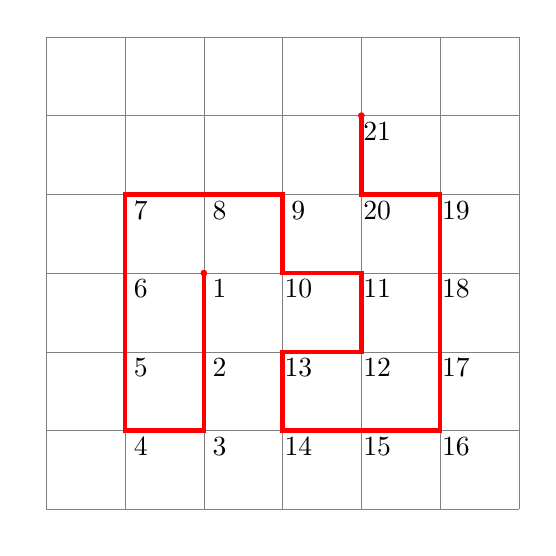
\begin{tikzpicture}[scale=1.00]
% grid
    \foreach \i in {\xMin,...,\xMax} {
        \draw [very thin,gray] (\i,\yMin) -- (\i,\yMax)  node [below] at (\i,\yMin) {};
    }
    \foreach \i in {\yMin,...,\yMax} {
        \draw [very thin,gray] (\xMin,\i) -- (\xMax,\i) node [left] at (\xMin,\i) {};
    }

% start and end of the self avoiding walk
\filldraw[red] (2,3) circle (1pt);
\filldraw[red] (4,5) circle (1pt);

% self avoiding walk
\draw[red, ultra thick] (2,3) -- (2,2) -- (2,1) -- (1,1) -- (1,2) -- (1,3) -- (1,4) -- (2,4) --
(3,4) -- (3,3) -- (4,3) -- (4,2) -- (3,2) -- (3,1) -- (4,1) -- (5,1) -- (5,2) -- (5,3) --
(5,4) -- (4,4) -- (4,5);

% self avoiding walk indexing
\node (A) at (2+\xshift,3+\yshift) {1};
\node (B) at (2+\xshift,2+\yshift) {2};
\node (C) at (2+\xshift,1+\yshift) {3};
\node (D) at (1+\xshift,1+\yshift) {4};
\node (E) at (1+\xshift,2+\yshift) {5};
\node (F) at (1+\xshift,3+\yshift) {6};
\node (G) at (1+\xshift,4+\yshift) {7};
\node (H) at (2+\xshift,4+\yshift) {8};
\node (I) at (3+\xshift,4+\yshift) {9};
\node (J) at (3+\xshift,3+\yshift) {10};
\node (K) at (4+\xshift,3+\yshift) {11};
\node (L) at (4+\xshift,2+\yshift) {12};
\node (M) at (3+\xshift,2+\yshift) {13};
\node (N) at (3+\xshift,1+\yshift) {14};
\node (O) at (4+\xshift,1+\yshift) {15};
\node (P) at (5+\xshift,1+\yshift) {16};
\node (Q) at (5+\xshift,2+\yshift) {17};
\node (R) at (5+\xshift,3+\yshift) {18};
\node (S) at (5+\xshift,4+\yshift) {19};
\node (T) at (4+\xshift,4+\yshift) {20};
\node (U) at (4+\xshift,5+\yshift) {21};



\end{tikzpicture} 
 \caption{Self-avoiding Walk}
 \label{fig:saw2}
\end{minipage}
\hspace{0.1\linewidth}
\begin{minipage}[b]{0.45\linewidth}
\centering
 \input{dec2}
 \caption{Edges marked with Over or Under}
 \label{fig:EOU}
\end{minipage}
\end{figure}


Let us consider the self avoiding walk in Fig. \ref{fig:saw2} as an example. Intuitively, a self-avoiding walk is said to have two ``sides". Contacts or edges that corresponds to the two sides (Over or Under) are said to form the two stacks and the contacts forming on differing sides (Over and Under) are said to form the queue. Each edge in the above self-avoiding walk is labeled $O$ or $U$ according to the following scheme:
\begin{noindlist}
  \item For non-walk edges adjacent to vertex $1$:
\begin{itemize}
  \item Among the two edges perpendicular to edge $\{1,2\}$, one is labeled $O$ and the other $U$.
  \item The remaining edge, if in the contact map, should be assigned the same label with which it forms a lattice square with the edges of the walk. Else it is labeled randomly.
\end{itemize}
  \item For non-walk edges adjacent to vertex $i$ where $2 \leq i \leq (n-1)$ the following rule is adopted:
	\begin{itemize}
  	  \item If the walk edge from vertex $(i-1)$ to vertex $i$ is in the same straight line, then at least one of the non-walk edges adjacent to $i$ and perpendicular to the edge $\{(i-1),i\}$ will be in the same lattice square with the edges marked at vertex $(i-1)$. In that case this new edge will have the same label.If that edge is labeled L then the other non-walk edge adjacent to $i$ would be labeled $\{O,U\}\setminus \{L\}$.
 	  \item If $i$ is a corner, the edges adjacent to it will share the same label. If any of the adjacent edges forms a lattice square with any edge of $(i-1)$, it will be labeled the same. Else (\emph{i.e.} when $(i-1)$ is also a corner) then edges adjacent to $i$ will be labeled the opposite label assigned to $(i-1)$.
	\end{itemize}
  \item For non-walk edges adjacent to vertex $n$:
\begin{itemize}
  	  \item   At least one of the non-walk edges adjacent to $n$ and perpendicular to the edge $\{(n-1),n\}$ will be in the same lattice square with the edges marked at vertex $(n-1)$. In that case this new edge will have the same label.If that edge is labeled L then the other non-walk edge adjacent to $n$ would be labeled $\{O,U\}\setminus \{L\}$.
 	  \item If the remaining edge adjacent to vertex $n$ is contained in the contact map, the same label is assigned as whichever of the two previously labeled edges is contained in the closed curve formed by the walk edges and the edge we are considering, else it is labeled arbitrarily.
	\end{itemize}
\end{noindlist}
Using the labeling scheme mentioned above, the self-avoiding walk in Fig. \ref{fig:saw2} can be labeled. The edges with two labels are only shown in Fig. \ref{fig:EOU} as they are the edges of the contact map. From Fig. \ref{fig:EOU}, it can be seen that there are three types of labeling of the edges with two labels in the graph - $\{O,O\}$, $\{U,U\}$ and $\{O,U\}$. Now we draw three graphs arranging the vertices in a linear scheme. The edges marked with $\{O,O\}$ will form one graph, the edges labeled $\{U,U\}$ the second graph and the edges labeled $\{O,U\}$ the third graph. Fig. \ref{fig:Two Stacks and the queue} shows the three graphs. It is clearly seen that two of them are stacks and the third one is a queue, thus proving the decomposition theorem.

\begin{figure}[ht]
\centering
\input{stack1}
 
\centering
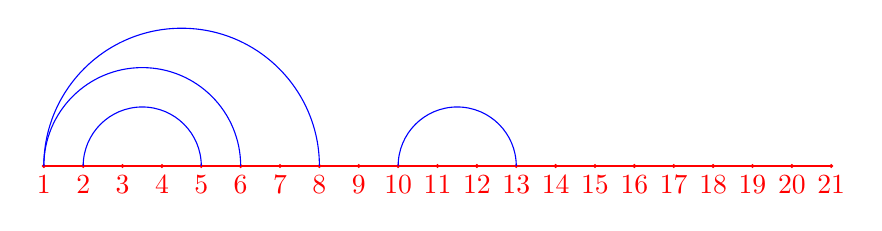
\begin{tikzpicture}[scale=0.5]


\foreach \i in {1,...,20} {
        \draw[red] (\i,1) -- (\i + 1,1)node[pos=0.0,below] {\i};
        \filldraw[red] (\i,1) circle (1pt);


 }

\draw[red] (21,1) -- (20,1)node[pos=0.0,below] {21};
\filldraw[red] (21,1) circle (1pt); 



\draw[blue, thin] (1,1) arc(180:0:3.5); 
\draw[blue, thin] (1,1) arc(180:0:2.5); 
\draw[blue, thin] (2,1) arc(180:0:1.5);
\draw[blue, thin] (10,1) arc(180:0:1.5);
\end{tikzpicture} 
\input{queue1}
\caption{Two Stacks and the queue}
 \label{fig:Two Stacks and the queue}
 \end{figure}

The decomposition theorem is considered an important step in formulating approximation algorithms for contact map overlap of self-avoiding walks. The first result in computing the contact map overlap is a $4$-approximation algorithm. Each walk in such setting is decomposed into two stacks and two staircases of maximum degree $2$. This is because each walk can be decomposed into two stacks and a queue and each queue can be decomposed into two staircases of maximum degree $2$. Polynomial time algorithms for these special cases are used to compute the 4-approximation algorithm. Considering the above decomposition theorem and with some minor modifications, it can further be shown that any contact map of a self-avoiding walk in two dimensional square lattice can be broken into one stack and two augmented staircases. This decomposition theorem is used to formulate the polynomial-time 3-approximation algorithm.

\citet{goip99} also state two very important open problems. One is to find better approximation ratio for contact map overlaps in two-dimensional lattice. The other is to find properties of three-dimensional self-avoiding walks and investigate if any approximation results can be obtained for the same. These two open problems are addressed in \citet{agmw07}. 